%; whizzy chapter
% -initex iniptex -latex platex -format platex -bibtex jbibtex -fmt fmt
% $B0J>e(B whizzytex $B$r;HMQ$9$k>l9g$N@_Dj!#(B

%     Kansai Debian Meeting resources
%     Copyright (C) 2007 Takaya Yamashita
%     Thank you for Tokyo Debian Meeting resources

%     This program is free software; you can redistribute it and/or modify
%     it under the terms of the GNU General Public License as published by
%     the Free Software Foundation; either version 2 of the License, or
%     (at your option) any later version.

%     This program is distributed in the hope that it will be useful,
%     but WITHOUT ANY WARRANTY; without even the implied warranty of
%     MERCHANTABILITY or FITNESS FOR A PARTICULAR PURPOSE.  See the
%     GNU General Public License for more details.

%     You should have received a copy of the GNU General Public License
%     along with this program; if not, write to the Free Software
%     Foundation, Inc., 51 Franklin St, Fifth Floor, Boston, MA  02110-1301 USA

%  preview (shell-command (concat "evince " (replace-regexp-in-string "tex$" "pdf"(buffer-file-name)) "&"))
% $B2hA|%U%!%$%k$r=hM}$9$k$?$a$K$O(Bebb$B$rMxMQ$7$F(Bboundingbox$B$r:n@.!#(B
%(shell-command "cd image200708; ebb *.png")

%%$B$3$3$+$i%X%C%@3+;O!#(B

\documentclass[mingoth,a4paper]{jsarticle}
\usepackage{kansaimonthlyreport}
\usepackage[dvips]{xy}
\usepackage{ulem}

% $BF|IU$rDj5A$9$k!"Kh7nJQ$o$j$^$9!#(B
\newcommand{\debmtgyear}{2013}
\newcommand{\debmtgdate}{24}
\newcommand{\debmtgmonth}{2}
\newcommand{\debmtgnumber}{69}

\begin{document}

\begin{titlepage}

% $BKh7nJQ99$9$kItJ,!"K\J8$NKvHx$b=$@5$9$k$3$H$r$o$9$l$:$K(B

 $BBh(B\debmtgnumber{}$B2s(B $B4X@>(B Debian $BJY6/2q;qNA(B

\vspace{2cm}

\begin{center}
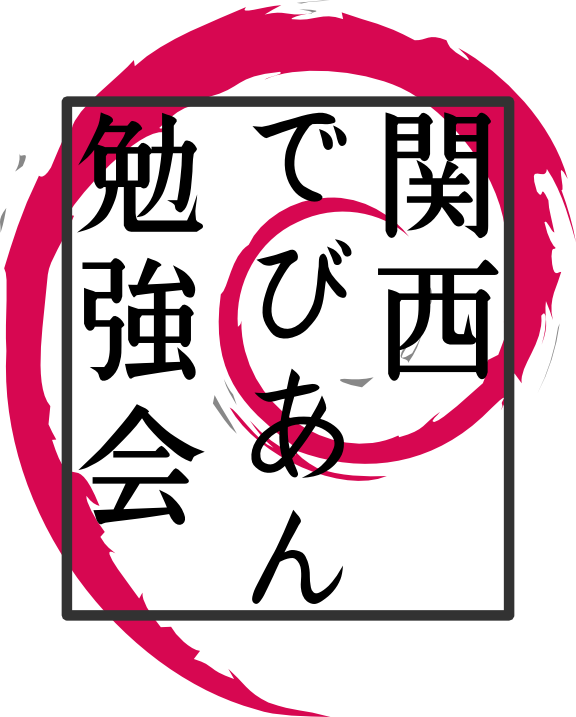
\includegraphics{image200802/kansaidebianlogo.png}
\end{center}

\begin{flushright}
\hfill{}$B4X@>(B Debian $BJY6/2qC4Ev<T(B $B:4!9LZ!&ARI_!&$N$,$?!&$+$o$@(B \\
\hfill{}\debmtgyear{}$BG/(B\debmtgmonth{}$B7n(B\debmtgdate{}$BF|(B
\end{flushright}

\thispagestyle{empty}
\end{titlepage}

\dancersection{Introduction}{Debian JP}

\vspace{1em}

 $B4X@>(BDebian$BJY6/2q$O(BDebian GNU/Linux$B$N$5$^$6$^$J%H%T%C%/(B
 ($B?7$7$$%Q%C%1!<%8!"(BDebian$BFCM-$N5!G=$N;EAH!"(BDebian$B3&7($G5/$3$C$?=PMh;v!"(B
 $B$J$I$J$I!K$K$D$$$FOC$79g$&2q$G$9!#(B

 $BL\E*$H$7$F<!$N;0$D$r9M$($F$$$^$9!#(B
 \begin{itemize}
  \item ML$B$d7G<(HD$G$O$J$/!"D>@\4i$r9g$o$;$k;v$G$N>pJs8r49$NB%?J(B
  \item $BDj4|E*$K=8$^$l$k>l=j(B
  \item $B;qNA$N:n@.(B
 \end{itemize}

 $B$=$l$G$O!"3Z$7$$0l;~$r$*3Z$7$_2<$5$$!#(B

\newpage

\begin{minipage}[b]{0.2\hsize}
 {\rotatebox{90}{\fontsize{80}{80}
{\gt $B4X@>(B Debian $BJY6/2q(B}}}
\end{minipage}
\begin{minipage}[b]{0.8\hsize}
\hrule
\vspace{2mm}
\hrule
\setcounter{tocdepth}{1}
\tableofcontents
\vspace{2mm}
\hrule
\end{minipage}

\dancersection{$B:G6a$N(BDebian$B4X78$N%$%Y%s%HJs9p(B}{Debian JP}

\subsection{$BBh(B 68 $B2s4X@>(B Debian $BJY6/2q(B}

68 $B2sL\$N4X@>(B Debian $BJY6/2q$O(B 1 $B7n(B 27 $BF|(B($BF|(B)$B$K9q:]F`NI3X%;%_%J!<%O%&%9(B
$B8&=$;\@_$G9T$J$o$l$^$7$?!#(B

$B5*Ln$5$s$N!V(BUsing Drupal on Debian$B!W$O!"(BDrupal $B$H(B Debian $B$N$*:nK!$N0c$$(B
$B$,$h$/$_$($k$h$$%;%C%7%g%s$G$7$?!#(B

$BLnJ}$5$s$N!V7n4)(B Debian Policy $B%*%Z%l!<%F%#%s%0%7%9%F%`!W$O0l2s$G<}$^$i(B
$B$J$$FbMF$@$C$?$N$GA0H>$N%f!<%6$H%0%k!<%W$^$G$H$J$j$^$7$?!#(Binit $B%9%/%j%W(B
$B%H0J9_$O<!2s$H$J$j$^$7$?$N$GB3$-$,3Z$7$_$G$9!#(B

$B=i$NF`NI3+:E$G$7$?$,!"2q>l$OF`NI8x1`Fb6a$/$NJ70O5$$N$h$$>l=j$G$7$?!#:#(B
$BG/$OBg:e0J30$N>l=j$G$bJY6/2q$r3+:E$7$?$$$G$9$M!#(B


\subsection{$BBh(B 97 $B2sEl5~%(%j%"(B Debian $BJY6/2q(B 2013$BG/(B2$B7nJY6/2q(B 2013 OSC$B=PD%(B}

97 $B2sL\$NEl5~%(%j%"(B Debian $BJY6/2q$O(B 2 $B7n(B 23 $BF|(B($BEZ(B)$B$K%*!<%W%s%=!<%9%+%s(B
$B%U%!%l%s%9(B 2013 Tokyo/Spring $B$K$F=PD%HG$H$7$F3+:E$5$l$^$7$?!#(B

$B%;%_%J!<$G$OLnEg$5$s$K$h$k!V(BDebian update - Debian$B$N:G?7F08~$K$D$$$F8l(B
$B$j$^$9!W$NH/I=$,9T$J$o$l$^$7$?!#(B

\subsection{$B%*!<%W%s%=!<%9%+%s%U%!%l%s%9(B 2013 Hamamatsu}
2 $B7n(B 9 $BF|(B($BEZ(B)$B$KIM>>;T;TL16(F/%;%s%?!<$G3+:E$5$l$?%*!<%W%s%=!<%9%+%s%U%!(B
$B%l%s%9(B 2013 Hamamatsu $B$KEl5~%(%j%"(B  Debian $BJY6/2q$G%V!<%9=PE8$7$^$7$?!#(B

\subsection{$BBh(B 1 $B2s(B Debian $B%Q%C%1!<%8%s%0F;>l(B}
2 $B7n(B 9 $BF|(B($BEZ(B)$B$K5~ETBg3X$GBh(B 1 $B2sL\$N(B Debian $B%Q%C%1!<%8%s%0F;>l$,3+:E$5(B
$B$l$^$7$?!#(B

$BEvF|$O(B 9 $BL>$N;22C<T$,8aA0Cf$K4d>>$5$s$+$i4pK\E*$J%Q%C%1!<%8$N:n@.J}K!$H(B
$B:G?7$N%Q%C%1!<%8%s%0;v>p$H;H$$J}$N@bL@$r$&$1!"8a8e$+$i3F<+$,;W$$;W$$$N(B
$B%Q%C%1!<%8:n@.$r9T$J$$$^$7$?!#(B

TitanPad $B$K;qNA$,$^$H$a$i$l$F$$$^$9$N$G;2>H$7$F$_$F$/$@$5$$!#(B
\url{http://debian-pkg-dojo.titanpad.com/1}

\dancersection{$B;vA02]Bj(B}{Debian JP}

$B:#2s$O0J2<$N2]Bj$r=PBj$7$^$7$?(B.
\begin{screen}
  \begin{enumerate}
  \item $B%j%j!<%9%N!<%H$N!VIUO?(B B. preseed $B$rMxMQ$7$?%$%s%9%H!<%k$N<+F02=!W(B\footnote{\url{http://www.debian.org/releases/stable/i386/apb.html.ja}}$B$rFI$s$G$-$F2<$5$$!#(B

    $B$^$?!"FI$s$G5$$K$J$kE@$J$I$,$"$l$P!"65$($F2<$5$$!#(B
  \item Wheezy $B$b$7$/$O(B sid $B4D6-$K(B apt-get install ruby $B$7$F$-$F2<$5$$!#(B
  \item $BIaCJ(B($B6HL3$b$7$/$O<qL#Ey(B)$B$*;H$$$N(B Ruby $B%=%U%H%&%'%"$,$"$l$P!"65$($F2<$5$$!#(B

    $B$^$?!"$=$l$,(B Debian $B%Q%C%1!<%8$K$J$C$F$$$J$$$J$i$P!"$4;XE&2<$5$$!#(B
  \end{enumerate}
\end{screen}

$B;22C<T$N3'$5$s$N2rEz$O0J2<$NDL$j$G$9!#(B

\begin{prework}{ $B@>;3OB9-(B }
  \begin{enumerate}
  \item $B$A$c$s$HFI$s$G$$$?$iD9$/$J$C$F$7$^$C$?$N$G(B \url{https://gist.github.com/znz/831f7bd6b0c5eff06530} $B$KCV$-$^$7$?!#(B

    \begin{itemize}
    \item[B.1.1.]
      hd-media $B$N(B hd $B$,2?$J$N$+5$$K$J$j$^$7$?!#(B
    \item[B.2.1.]
      $B%$%s%9%H!<%i$,3N<B$K@5$7$$;vA0@_Dj%U%!%$%k$r<hF@$9$k$N$K!"$3$N%U%!%$%k$N%A%'%C%/%5%`$r;XDj$G$-$^$9!#8=:_!"$3$l$K$O(B md5sum $BCM$N;XDj$,I,MW$G$9!#;XDj$7$?CM$H;vA0@_Dj%U%!%$%k$NCM$O0lCW$7(B
      $B$J$1$l$P$J$j$^$;$s!#0lCW$7$J$$>l9g$O!"%$%s%9%H!<%i$O;vA0@_Dj%U%!%$%k$r;HMQ$7$^$;$s!#(B
   
      $BI,?\$+$I$&$+$o$+$j$K$/$$$H;W$$$^$7$?!#(B
    \item[B.2.2.]
      $BCm0U(B

      $B8=:_$N(B Linux $B%+!<%M%k(B (2.6.9 $B0J9_(B) $B$G$O!":GBg(B ($B%$%s%9%H!<%i$,%G%U%)%k%H$G;XDj$9$k%*%W%7%g%s$r4^$a(B) $B%3%^%s%I%i%$%s%*%W%7%g%s$r(B 32 $B8D!"4D6-%*%W%7%g%s$r(B 32 $B8D<u$1<h$l$^$9!#$3$N?t$rD6$((B    $B$k$H!"%+!<%M%k$O%Q%K%C%/(B ($B%/%i%C%7%e(B) $B$7$F$7$^$$$^$9(B ($B0JA0$N%+!<%M%k$G$O$3$N?t;z$,$b$C$H>/$J$$$G$9(B)$B!#(B
   
      $BD9$5$N@)8B$,$"$k$N$+$I$&$+5$$K$J$j$^$7$?!#(B

    \item[B.2.3.]
    auto $B%V!<%H%i%Y%k$O!"$^$@$I$3$K$bDj5A$5$l$F$$$^$;$s!#(B
   
    $B!V(Bauto url=...$B!W$H$$$&$N$,;H$($k$N$+$I$&$+$o$+$j$^$;$s$G$7$?!#(B

    \item[B.2.5.]
    $B$3$NJ8;zNs$G!"%M%C%H%o!<%/>e$NA4%^%7%s$K(B preseed $B$G%$%s%9%H!<%k$9$k$N$G$O$J$/!"FCDj$N%[%9%H$KBP$7$F9T$&$h$&$K$b$G$-$^$9!#(B
   
    $B$3$NJ8;zNs$H$O(B?

    \item[B3]
    $B7?$HCM$N4V$O$h$/$"$j$^$;$s!#(B
   
    $B7?$O%?%$%W(B ($B<ALd%?%$%W(B) $B$G$7$g$&$+(B?

    \item[B.4.1. $BCO0h2=(B]
    $B$3$NJ}K!$OHqMQ$K;H$&$N$,MF0W$G$9$,!"8@8l!"9q!"%m%1!<%k$NMxMQ2DG=$JAH$_9g$o$;$r$9$Y$F(B preseed $B$G$-$k$o$1$G$O$"$j$^$;$s(B[29]$B!#8@8l$H9q$O!"$I$A$i$b%V!<%H%Q%i%a!<%?$G;XDj$G$-$^$9!#(B
   
    $BHqMQ$K;H$&$N$,MF0W$H$$$&$H$3$m$N0UL#$,J,$+$j$^$;$s$G$7$?!#(B

    \item[B.4.5.]
    $B%Q%9%o!<%I$rCN$C$F$$$k;vA0@_Dj%U%!%$%k$,C/$G$b%"%/%;%9$G$-$k$?$a$K!"(B
   
    $B!V;vA0@_Dj%U%!%$%k$,!W$O!V;vA0@_Dj%U%!%$%k$O!W$H$+!V;vA0@_Dj%U%!%$%k$r!W$H$+$NJ}$,NI$$$N$G$O$J$$$G$7$g$&$+!#(B

    \item[B.4.10.]
    $B$3$N%Q%i%a!<%?$NCM$O!"%+!<%M%k%3%^%s%I%i%$%s$K$=$N$^$^EO$5$l$k$N$G!"%+%s%^$+6uGr$G6h@Z$C$?%Q%C%1!<%8$N%j%9%H$r<h$l$^$9!#(B
   
    $B%+!<%M%k%3%^%s%I%i%$%s$G$OCM$K6uGr6h@Z$j$O;H$($J$$$O$:$J$N$G!"8mLu$N$h$&$K8+$($^$9!#(B

    \item[B.5.2.]
    $B$3$N>l9g$G$b<ALd$O9T$o$l$^$9!#(B
   
    $B$3$3$b8mLu$G$7$g$&$+(B? $B1Q8l$NJ}$O!V<ALd:Q$_>uBV$N$^$^!W(B($B$@$+$i<ALd$5$l$J$$(B) ($B$N$G8eB3$NJ8$GL$<ALd>uBV$KLa$9!"$HB3$/(B) $B$H$$$&0UL#$K8+$($^$9!#(B

    \item[B.5.2.]
    $BGI%1!<%8(B
   
    typo?

    \item[B.5.3.]
    $BB>$N%U%!%$%k$G$h$j3N$+$J@_Dj$r;XDj$9$k(B
   
    specific $B$r!V3N$+$J!W$HLu$9$N$O$A$g$C$H0c$&$h$&$K46$8$^$7$?!#(B

  \end{itemize}

  \item $B%$%s%9%H!<%k$7$^$7$?!#(B
  \item nadoka $B$H$$$&(B IRC $B$N(B proxy $B$N$h$&$J$b$N$r;H$C$F$$$k$N$G$9$,!"?7$7$$%P!<%8%g%s$,(B Debian $B%Q%C%1!<%8$K$J$C$F$$$^$;$s!#(B
  \end{enumerate}
\end{prework}

\begin{prework}{ $B$+$o$@$F$D$?$m$&(B }
  \begin{enumerate}
  \item $BFI$s$G$_$^$7$?!#(B

    preseed $B$r;H$C$?$3$H$O$J$$$N$G$9$,!"7Y9p$,$"$k$h$&$K%Q!<%F%#%7%g%sJ,3d$,$O$^$j$=$&$J5$$,$7$^$9!#(B
  \item $B$7$F$"$j$^$9!#(B
  \item redmine, nokogiri, rabbit
  \end{enumerate}
\end{prework}

\begin{prework}{ $B;3>k$N9q$N=;?M(B $B5WJ]Gn(B }
  \begin{enumerate}
  \item $B$O$$!":#$+$i4hD%$j$^$9!#(B
  \item $B$O$$!#(Bschroot $B$NCf$K:n$C$?(B sid $B4D6-$K%$%s%9%H!<%k$7$F$*$-$^$9!#(B
  \item Redmine $B$r;H$C$F$$$^$9!#(B
  \end{enumerate}
\end{prework}

\begin{prework}{ murase\_{}syuka }
  \begin{enumerate}
  \item $B7Z$/FI$s$G$_$?$,NI$/J,$+$i$J$$(B
  \item rvm$B$G(Binstall$B:Q$_(B
  \item rvm/irb(pry)/rails
  \end{enumerate}
\end{prework}

\begin{prework}{ $B$N$,$?$8$e$s(B }
  \begin{enumerate}
  \item $B$O$$FI$_$^$7$?!#$,!"$$$^$@$K(BHDD$B$N%Q!<%F%#%7%g%s$N@Z$jJ}$,$h$/$o$+$C$F$J$+$C$?$j!#(B

    \url{http://www.nofuture.tv/linux/debianautoinstall}
  \item $B$O$$!#F~$C$F$^$9!#(B
  \item tDiary$B$r;H$C$F$^$9(B
  \end{enumerate}
\end{prework}

\begin{prework}{ $B$h$7$@$H$b$R$m(B }
  \begin{enumerate}
  \item $BFI$s$G$*$-$^$9!#(B
  \item sid$B4D6-$G!"(Bapt-get install ruby $B<B9T$7$^$7$?!#(B
  \item rabbit$B$/$i$$$+$b!#(B
  \end{enumerate}
\end{prework}

\begin{prework}{ yyatsuo }
  \begin{enumerate}
  \item $B0lDL$jFI$s$G$_$^$7$?(B
  \item Ruby 1.9.1 $B%$%s%9%H!<%k:Q$_$G$9(B
  \item $BIaCJ;H$&$N$O(B RedMine

    $B:#$^$G$K;H$C$?$3$H$,$"$k$N$O(B Milkode $B$H(B Termtter
  \end{enumerate}
\end{prework}

\begin{prework}{ $B:4F#@?(B }
  \begin{enumerate}
  \item $B:#FI$s$G$^$9!#(B

    $B$A$g$C$H;n$7$F$_$?$$$1$I!";~4V$,(B...($B4@(B
  \item $B2>A[4D6-$N(Bsqueeze$B$r!":rHU$h$&$d$/(Bwheezy$B$K$"$2$^$7$?!#(B

    $B$(!<$H!"(Bruby $B$bF~$C$F$k$O$:(B($BL$3NG'(B)
  \item tdiary$B$G%V%m%0$r=q$$$F$$$^$9!#(B
  \end{enumerate}
\end{prework}

\begin{prework}{ $B:4!9LZMNJ?(B }
  \begin{enumerate}
  \item preceed $B$h$/;H$C$F$^$9(B
  \item $BIaCJ$+$i;H$C$F$^$9!#$=$m$=$m(B mruby $B$H(B ruby2.0 $B$rF~$l$?$$$G$9$M!#(B
  \item redmine $B$H(B Jekyll $B$,$J$$$HESJ}$K$/$l$^$9!#$"$H!":#2s$N%W%l%<%s$O(B rabbit $B$G$9!#(B
  \end{enumerate}
\end{prework}

\begin{prework}{ $BBgNS(B }
  \begin{enumerate}
  \item $B0lDL$jFI$_$^$7$?!#(B
  \item Wheezy$B$N<B83MQ4D6-$K%$%s%9%H!<%k$7$^$7$?!#(B

    $B$?$@%M%C%H%o!<%/$N8~$3$&B&$N(BVM$B$N>e$J$N$G!"2q>l$G$O;H$($J$$$+$b$7$l$^$;$s!#(B

    $B2q>l$G%M%C%H%o!<%/$,$b$7;H$($l$P$$$1$k$N$G$9$,!#(B
  \item yard, rmagick, test-unit, NArray, depq $B$J$I(B
  \end{enumerate}
\end{prework}

\begin{prework}{ kazuhito.sumpic }
($BL52sEz(B)
\end{prework}

\dancersection{Debian Installer $B%H%i%V%k%7%e!<%F%#%s%0(B}{Yuryu}

\subsection{$B<+8J>R2p(B}
\begin{itemize}
\item Yuryu (twitter: @Yuryu)
\item $BK?<R$G%$%s%U%i%(%s%8%K%"$7$F$^$9(B
\item potato $B"*(B woody $B"*(B ($BIb5$(B) $B"*(B Ubuntu(Gusty) $B"*(B ... $B"*(B Ubuntu(Precise)
\item $B2q<R$G$O(B Debian $B;H$C$F$^$9(B
\item $B9%$-$J%3%^%s%I$O(B xargs
\end{itemize}

\subsection{Preseed}
\subsubsection{Preseed $B$H$O(B}
\begin{itemize}
\item Debian Installer $B$N1~Ez%U%!%$%k(B
\item $B$9$Y$F$NA*Br;h$,A*$Y$k(B
\item PXE $B$HAH$_9g$o$;$k$H6/$$(B
\item $BC1BN$G$b;H$($^$9(B($B>/!9LLE](B)
\end{itemize}

\begin{commandline}
locale=en_US language=en country=JP
console-keymaps-at/keymap=jp106
keyboard-configuration/xkb-keymap=jp106
interface=eth0 hostname=debian
domain=local url=http://holo.yuryu.jp/
preseed.cfg DEBCONF_DEBUG=5
\end{commandline}

\subsubsection{boot$B%*%W%7%g%s$NI,MW@-(B}
\begin{itemize}
\item Preseed $B%U%!%$%k$,FI$^$l$k$N$O!"%M%C%H%o!<%/$N@_Dj$,=*$o$C$F$+$i(B
\item $B%M%C%H%o!<%/@_DjA0$K$b%$%s%9%H!<%i!<$N<ALd$O$"$k(B
\item $B"*%V!<%H%*%W%7%g%s$H$7$FEO$9(B
\item $BD9$$$N$G<jBG$A$OL5M}!"(BPXE $B$r;H$&(B
\end{itemize}

\subsubsection{expert install}
\begin{itemize}
\item expert options $B"*(B automated install
\item $BESCf$G(B preseed $B%U%!%$%k$r;XDj$G$-$k(B
\item $B$H$j$"$($:;n$9$K$O$3$C$A(B
\end{itemize}

\subsubsection{url}
\begin{itemize}
\item preseed $B%U%!%$%k$N>l=j(B
\item http, ftp, tftp $B$G;XDj(B
\item https $B$O;H$($J$$(B(!)
\end{itemize}

\subsubsection{$B%U%!%$%k$NCf?H(B}
\begin{itemize}
\item $B!V(Bd-i $B9`L\L>(B $B;XDj!W$NMeNs(B
\end{itemize}

\begin{commandline}
### Clock and time zone setup
# Controls whether or not the hardware clock is set to UTC.
d-i clock-setup/utc boolean true

# You may set this to any valid setting for $TZ; see the contents of
# /usr/share/zoneinfo/ for valid values.
d-i time/zone string Asia/Tokyo

# Controls whether to use NTP to set the clock during the install
d-i clock-setup/ntp boolean true
# NTP server to use. The default is almost always fine here.
d-i clock-setup/ntp-server string ntp.nict.go.jp
\end{commandline}
%$

\subsubsection{$B%U%!%$%k$N=q$-J}(B}
\begin{itemize}
\item $B4pK\E*$K$O%5%s%W%kDL$j(B
\item $B$G$b!"$$$/$D$+Mn$H$77j$,(B...
  \begin{itemize}
  \item $B0lHVBgJQ$J$N$,(B partitioning
  \end{itemize}
\end{itemize}

\subsection{partitioning}

\subsubsection{partitioning}
\begin{itemize}
\item d-i partman-auto/choose\_recipe
  \begin{itemize}
  \item atomic - / $B0lH/(B
  \item home - /home $B$@$1J,$1$k(B
  \item multi - /home, /usr, /var, /tmp
  \end{itemize}
\item d-i partman-auto/expert\_recipe
\end{itemize}

\subsubsection{recipe}
\begin{commandline}
d-i partman-auto/expert_recipe string                         \
      boot-root ::                                            \
              40 50 100 ext2                                  \
                      $primary{ } $bootable{ }                \
                      method{ format } format{ }              \
                      use_filesystem{ } filesystem{ ext2 }    \
                      mountpoint{ /boot }                     \
              .                                               \
              500 10000 -1 ext4                               \
                      method{ format } format{ }              \
                      use_filesystem{ } filesystem{ ext4 }    \
                      mountpoint{ / }                         \
              .                                               \
              64 512 300% linux-swap                          \
                      method{ swap } format{ }                \
              .
\end{commandline}

\clearpage

\subsubsection{$B%l%7%T7A<0(B}

$B%l%7%TL>(B ::

\ $B:GDcMFNL(B(MB) $BM%@hEY(B $B:GBgMFNL(B FS

\ $B%Q!<%F%#%7%g%sFbMF(B .

\begin{commandline}
 500 1000 -1 ext4 \
 method{ format } format{ } \
 use_filesystem{ } filesystem{ ext4 } \
 mountpoint{ /home }
\end{commandline}

\subsubsection{$BMFNL(B}
\begin{itemize}
\item $B:GBg$r(B -1 $B$K$9$k$H6u$-MFNL$r$9$Y$F;H$&(B
\item $BM%@hEY$O?t;z$,Bg$-$J$[$&$,Dc$$(B
\item $B:G>.(B=$B:GBg$K$;$:(B100MB$BDxEY$NI}$r$b$?$;$k(B
\end{itemize}

\subsubsection{method}
\begin{itemize}
\item format
  \begin{itemize}
  \item $BDL>oDL$j%U%)!<%^%C%H$7$F;HMQ(B
  \end{itemize}
\item swap
  \begin{itemize}
  \item $B%9%o%C%W%Q!<%F%#%7%g%s$H$7$F;HMQ(B
  \end{itemize}
\item keep
  \begin{itemize}
  \item $B2?$b$;$:6h2h$@$1:n$k(B
  \end{itemize}
\end{itemize}

\subsubsection{$B%U%!%$%k%7%9%F%`(B}
\begin{itemize}
\item $BMFNL$N1&B&$K=q$/$b$N$H!"(Bfilesystem\{ \}
\item $B4pK\E*$K$OF1$8(B
\item ext[2-4], xfs, btrfs, jfs, linux-swap
\item keep $B$N$H$-$OL5;k$5$l$k(B(free $B$G$b(Bok)
\end{itemize}

\subsubsection{$B$*LsB+(B}
\begin{itemize}
\item $B>iD9$K8+$($F$b!">JN,$G$-$J$$$b$N(B
\item format\{ \}
\item use\_filesystem\{ \}
\item filesystem\{ ext4 \}
\end{itemize}

\subsection{$B%O%^$j$^$7$?(B}

\subsubsection{primary}
\begin{itemize}
\item \$primary\{ \} $B%W%i%$%^%jI,?\;XDj(B
\item \$logical\{ \} $B$b$"$j$=$&(B?
  \begin{itemize}
  \item $B<B$OL5$$(B
  \item $B>JN,$9$k$H(B logical $B$K$J$k(B
  \end{itemize}
\end{itemize}

\subsubsection{$B0l9T$G=q$/(B}
\begin{itemize}
\item $B9TKv$K(B \textbackslash $B$r=q$$$F!"0l9T$K$D$J$2$F=q$/(B
\item \textbackslash $B$N8e$K%9%Z!<%9$,$"$k$H$=$3$G@Z$l$^$9(B
\end{itemize}
 
\subsubsection{$B%l%7%TL>(B}
\begin{itemize}
\item $B%l%7%TL>$,I,?\(B
\item partman-auto/choose\_recipe $B$H$OL54X78(B
  \begin{itemize}
  \item expert recipe $B;H$&$J$i=q$$$F$O$$$1$J$$(B
  \end{itemize}
\item $B2?$r=q$$$F$bF0:n$K4X78$J$7(B...
\end{itemize}

\begin{commandline}
d-i partman-auto/expert_recipe string                         \
      boot-root ::                                            \
\end{commandline}

\subsubsection{$B%9%Z!<%9$N07$$(B}
\begin{itemize}
\item $B4pK\E*$K$O%9%Z!<%9I,?\(B
\item $B3+$-%+%C%3$N<jA0$O%9%Z!<%9IT2D(B
  \begin{itemize}
  \item $B!{(B method\{\_format\_\}
  \item $B!_(B method\_\{\_format\_\}
  \end{itemize}
\item grep $B$G%Q!<%9$7$F$k$N$G873J$G$9(B...
\end{itemize}

\subsubsection{$B%l%7%T!"G'<1$5$l$F$k(B?}
\begin{itemize}
\item /tmp/expert\_recipe
\item $B<B:]$K;H$o$l$?%l%7%T$,F~$k(B
\end{itemize}

\subsection{$B$=$NB>(Btroubleshoot}
\subsubsection{d-i $B$8$c$J$$9T$b$"$k(B}
\begin{itemize}
\item d-i $B$G;O$^$i$J$$9T$b$"$k(B
\item tasksel
  \begin{itemize}
  \item popularity-contest
  \item $B%3%T%Z;v8N$KCm0U(B
  \end{itemize}
\end{itemize}

\subsubsection{$B;_$^$C$?$i(B}
\begin{itemize}
\item syslog $B$r3NG'(B
\item INPUT ... $B$N9T$,%Q%i%a!<%?!<L>(B
\end{itemize}

\subsubsection{$B%m%0(B}
\begin{itemize}
\item Alt+F4 $B$N%m%0(B
\item $B%$%s%9%H!<%kCf(B /var/log/syslog
\item $B%$%s%9%H!<%k8e(B /var/log/installer/syslog
\item DEBCONF\_DEBUG $B$,I,?\(B
\end{itemize}

\subsubsection{$B$3$o$/$J$$$h(B}
\begin{itemize}
\item debian installer $B$N<BBV$O%7%'%k%9%/%j%W%H(B
\item $B3F%G%#%l%/%H%j$r(B for $B$G=g$K8F$s$G$k(B
\item $B9`L\L>$G(B grep $B$7$F$_$k$H%R%s%H$,(B
\end{itemize}

\subsubsection{debian/*.templates}
\begin{itemize}
\item debian-installer $B$N3F<o%Q%C%1!<%8$N(B debian/*.templates
\item $BJQ?tL>!"7?!"@bL@$,B7$C$F$k(B
\item $B%j%U%!%l%s%9Be$o$j$K$J$j$^$9(B
\end{itemize}

\begin{commandline}
Template: partman-partitioning/bootable_logical
Type: boolean
Default: false
# :sl2:
_Description: Are you sure you want a bootable logical partition?
 You are trying to set the bootable flag on a logical partition. The
\end{commandline}

\subsubsection{debconf-get-selections}
\begin{itemize}
\item $B%$%s%9%H!<%k:Q$_(BOS$B$+$i@_Dj$r<hF@(B
\item debconf-get-selections --installer
\item $B%G%U%)%k%HCM$b4^$a$FBgNL$K=P$k(B
  \begin{itemize}
  \item $BI,MW$JJ*$r<h<NA*Br$9$kI,MW$"$j(B
  \end{itemize}
\end{itemize}

\subsubsection{Ubuntu $BBP1~(B}
\begin{itemize}
\item $B4pK\E*$K$OF1$8(B
\item $B$$$/$D$+DI2C$N<ALd(B
  \begin{itemize}
  \item d-i pkgsel/update-policy select none
  \item d-i user-setup/allow-password-weak boolean true
  \item d-i user-setup/encrypt-home boolean false
  \end{itemize}
\item $B>\$7$/$O(B \url{https://help.ubuntu.com/lts/installation-guide/i386/preseed-contents.html}
\end{itemize}

\subsection{$B$^$H$a(B}
\begin{itemize}
\item $B:$$C$?$i(B syslog $B$r4Q$k(B
\item recipe $B$O%9%Z!<%9$K5$$r$D$1$k(B
\item DEBCONF\_DEBUG=5 $B=EMW(B!
\end{itemize}

\clearpage

\dancersection{Ruby In Wheezy}{$B:4!9LZMNJ?(B}

\vspace{1em}

$B<!4|0BDjHG(B Debian 7.0 (Wheezy) $B$K$*$1$k(B Ruby $B4D6-$K$D$$$F!"(B%
$BFC$KJ#?t$N(B Ruby $B<BAu$N6&B8$H(B Gem $B$H$N$*IU$-9g$$$N;EJ}$K$D$$$F!"(B
$B4JC1$K$*OC$7$7$^$9!#(B

\subsection{``Ruby'' in Wheezy}

Ruby $B$K$OJ#?t$N<BAu$,B8:_$7$F$$$^$9!#(B
Debian Wheezy $B$G$O0J2<$N(B Ruby $B%$%s%?!<%W%j%?$,;HMQ$G$-$^$9(B:
\begin{table}[h!]
  \centering
  \begin{tabular}{lll}
    $B%$%s%?!<%W%j%?(B & $B%Q%C%1!<%8L>(B       & $BCm0U=q$-(B \\
    MRI 1.8.7      & \texttt{ruby1.8}   &          \\
    MRI 1.9.3      & \texttt{ruby1.9.3} & \texttt{ruby1.9.1} $B%Q%C%1!<%8$N<BBV$O(B \texttt{ruby1.9.3} $B$@$C$?$j$7$^$9!#(B \\
    JRuby          & \texttt{jruby}     & $B%Q%C%1!<%8$O(B Debian Java Maintainers $B$K$h$C$F4IM}$5$l$F$$$^$9(B \\
    Rubinius       & \texttt{rubinius}  & $B8=:_:n6HCf$G$9(B. ITP\#591817 \\
    mruby          & \texttt{mruby}     & $B8=:_:n6HCf$G$9(B. ITP\#697835 \\
  \end{tabular}
\end{table}
%
\newline
$B!V(B\texttt{ruby1.9.1} $B%Q%C%1!<%8$N<BBV$O(B \texttt{ruby1.9.3} $B$@$C$?$j$7$^$9!#!W$K$D$$$F!"(B
Ruby $B$N(B soname $B$,JQ$o$C$F$$$J$$$N$G(B \texttt{libruby1.9.1} $BEy$N%Q%C%1!<%8$,;D$C$F$*$j!"(B
\texttt{ruby1.9.3} $B%Q%C%1!<%8$O(B \texttt{/usr/bin/ruby1.9.1} $B$X$N(B
symbolic link $B$rDs6!$9$k$@$1$@$C$?$j$7$^$9!#(B
\begin{commandline}
% dpkg -S ruby1.9.3
ruby1.9.3: /usr/bin/ruby1.9.3
ruby1.9.3: /usr/share/man/man1/ruby1.9.3.1.gz
ruby1.9.3: /usr/share/doc/ruby1.9.3
ruby1.9.3: /usr/share/doc/ruby1.9.3/NEWS.Debian.gz
ruby1.9.3: /usr/share/doc/ruby1.9.3/NEWS.gz
ruby1.9.3: /usr/share/doc/ruby1.9.3/changelog.Debian.gz
ruby1.9.3: /usr/share/doc/ruby1.9.3/changelog.gz
ruby1.9.3: /usr/share/doc/ruby1.9.3/copyright
ruby1.9.3: /usr/share/doc/ruby1.9.3/README.gz
% ls -la /usr/bin/ruby1.9.3
lrwxrwxrwx 1 root root 9 Feb 23 23:44 /usr/bin/ruby1.9.3 -> ruby1.9.1*
\end{commandline}
$BB>$K$b!"(B\texttt{Topaz} $B$d(B \texttt{HPC Ruby Compiler} $B$J$I!"(B($B8D?ME*$K(B)$B5$$K$J$k<BAu$,$"$j$^$9$,!"$^$@(B Debian $B$G$I$&$3$&$H$$$&$*OC$K$O$J$C$F$$$^$;$s!#(B

\subsection{$BJ#?t$N(B Ruby $B<BAu$N@Z$jBX$((B}

$B$5$F(B, $B$3$l$@$1J#?t$N(B Ruby $B<BAu$,$"$k$H!"$=$l$r@Z$jBX$($F;H$$$?$/$J$k$N$,?M>p$@$H;W$$$^$9!#(B
Debian $B$K$O!"F1$85!G=$rDs6!$9$k%=%U%H%&%'%"$r$-$j$+$($k(B \texttt{update-alternatives} $B$H$$$&;EAH$_$,4{$K$"$j$^$9!#(B
$B$G$9$,!"(B\texttt{/usr/bin/ruby} $B$r@Z$jBX$($?$i(B \texttt{gem} $B$d(B \texttt{irb} $B$J$s$+$b@Z$jBX$($?$/$J$k$G$7$g$&!#(B
$B$=$N$?$a!"$3$l$i$r0lEY$KJQ49$9$k$?$a$N%3%^%s%I$,Ds6!$5$l$F$$$^$9!#(B

\subsubsection{$B%7%9%F%`A4BN$G%G%U%)%k%H$N(B Ruby $B$r@Z$jBX$($k$K$O(B?: \texttt{ruby-switch}}

$B%7%9%F%`A4BN$G%G%U%)%k%H$N(B Ruby $B%$%s%?!<%W%j%?$rA*Br$9$k$?$a$K!"(Bruby-switch $B%Q%C%1!<%8$,;HMQ2DG=$G$9!#(B $B$3$l$O(B root $B$H$7$F(B($B$b$7$/$O(B sudo $B$r;H$C$F(B)$B<B9T$9$kI,MW$,$"$j$^$9!#(B
\begin{commandline}
# ruby -v
ruby 1.8.7 (2011-06-30 patchlevel 352) [x86_64-linux]
# ruby-switch --list
ruby1.8
ruby1.9.1
# ruby-switch --set ruby1.9.1
update-alternatives: using /usr/bin/gem1.9.1 to provide /usr/bin/gem (gem) in manual mode.
update-alternatives: using /usr/bin/ruby1.9.1 to provide /usr/bin/ruby (ruby) in manual mode.
# ruby -v
ruby 1.9.3p0 (2011-10-30 revision 33570) [x86_64-linux]
# ruby-switch --auto
update-alternatives: using /usr/bin/ruby1.8 to provide /usr/bin/ruby (ruby) in auto mode.
update-alternatives: using /usr/bin/gem1.8 to provide /usr/bin/gem (gem) in auto mode.
# ruby -v
ruby 1.8.7 (2011-06-30 patchlevel 352) [x86_64-linux]
\end{commandline}

\subsubsection{$B%f!<%6Kh$K%G%U%)%k%H$N(B Ruby $B%$%s%?!<%W%j%?$rA*Br$9$k$K$O(B: \texttt{rbenv}}

$B%f!<%6%"%+%&%s%HKh$K%G%U%)%k%H$N(B Ruby $B%$%s%?!<%W%j%?$r@Z$jBX$($k$K$O!"(Brbenv $B%Q%C%1!<%8$r;H$&$N$,NI$$$G$7$g$&!#(B
\begin{commandline}
% ruby -v
ruby 1.8.7 (2011-06-30 patchlevel 352) [x86_64-linux]
% rbenv init
# Load rbenv automatically by adding
# the following to ~/.bash_profile:

eval ``$(rbenv init -)"
% echo 'eval ``$(rbenv init -)"' >> ~/.bash_profile # or ~/.bashrc, depends on your setup
% rbenv versions
% rbenv alternatives
% rbenv versions
  1.8.7-debian
  1.9.3-debian
% rbenv global 1.9.3-debian
% ruby -v
ruby 1.8.7 (2011-06-30 patchlevel 352) [x86_64-linux]
\end{commandline}
%%$
$B0l8+$A$c$s$HF0:n$7$F$$$J$$$h$&$K8+$($^$9$,!"$3$l$O8=:_<B9TCf$N%7%'%k$,(B "ruby" $B$N0LCV$H$7$F(B /usr/bin/ruby $B$r%-%c%C%7%e$7$F$$$k$+$i$G$9!#?7$7$$%7%'%k$r3+;O$7$?8e$K$O!"%G%U%)%k%H$N(B Ruby $B$r9T$C$?$jMh$?$j@Z$jBX$($k$3$H$,$G$-$^$9!#(B
\begin{commandline}
% ruby -v
ruby 1.8.7 (2011-06-30 patchlevel 352) [x86_64-linux]
% rbenv global 1.9.3-debian
% ruby -v
ruby 1.9.3p0 (2011-10-30 revision 33570) [x86_64-linux]
% rbenv global 1.8.7-debian
% ruby -v
ruby 1.8.7 (2011-06-30 patchlevel 352) [x86_64-linux]
\end{commandline}

\subsubsection{Debian $B%Q%C%1!<%8$K$J$C$F$$$J$$(B Ruby $B$r%$%s%9%H!<%k$9$k$K$O(B: \texttt{ruby-build}}

\texttt{ruby-build} $B$r;HMQ$9$k$3$H$G!"(BDebian $B$G$^$@;HMQ2DG=$K$J$C$F$$$J$$(B Ruby $B%$%s%?!<%W%j%?$r%$%s%9%H!<%k$9$k$3$H$,$G$-$^$9!#(B
$B$7$+$7$J$,$i!"$3$N%Q%C%1!<%8$N(B README.Debian $B%U%!%$%k$K=q$+$l$F$$$kFbMF$KCm0U$7$F2<$5$$(B:
\begin{commandline}
  While ruby-build is a great tool to build Ruby versions that are not
  available via APT, you should still use the Debian-packaged versions
  of Ruby whenever possible since they are tested and supported by the
  Debian community.

  Please do not report bugs you encounter while using your homebuilt
  Rubies to the Debian team; Rubies built by yourself are not supported.
\end{commandline}
% $B$H$O$$$((B \texttt{ruby2.0} $B$,$=$m$=$m=P$^$9$7!"(B\texttt{ruby-build} $B$r;H$&?M$bB?$$$H;W$$$^$9(B.
% \footnote{$B8D?ME*$K$O(B \texttt{backports} $B$9$kM=Dj$G$9$,(B.}.
$B$H$$$&$o$1$G!">\:Y$O(B \texttt{man ruby-build} $B$H$$$&$3$H$G!#(B

\subsection{Debian $B$K$*$1$k(B Ruby $B%Q%C%1!<%8%s%0(B}

Debian $B$G$O(B Ruby $BK\BN$N%Q%C%1!<%8%s%0$O(B \texttt{pkg-ruby} $B%A!<%`!"(B
Gem $BEy$GG[I[$5$l$F$$$k(B($B3HD%(B)$B%i%$%V%i%j$d%"%W%j%1!<%7%g%s$O(B
\texttt{pkg-ruby-extras} $B%A!<%`$K$h$C$F%a%s%F$5$l$F$$$^$9!#(B
$B<!$NOCBj$O(B
\texttt{pkg-ruby-extras} $B%A!<%`$,NI$/$d$C$F$$$k$3$H!"(B
$B$9$J$o$A(B Gem $B$GG[I[$5$l$F$$$k(B Ruby ($B3HD%(B)$B%i%$%V%i%j$N(B Debian $B%Q%C%1!<%82=$K$D$$$F!"$G$9!#(B

\subsection{Gem $B%Q%C%1!<%8$r(B Debian $B%Q%C%1!<%8$K(B: \texttt{gem2deb}}

Gem $B$GG[I[$5$l$F$$$k(B Ruby ($B3HD%(B)$B%i%$%V%i%j$O(B
\texttt{gem2deb} $B$rMQ$$$k$3$H$G(B Debian $B%Q%C%1!<%8$KJQ492DG=$G$9!#(B\textbf{$B$?$$$F$$$N>l9g$O(B}$B!#(B
\texttt{gem2deb} $B$K$h$k$*<j7Z%Q%C%1!<%8%s%0$N@.8yN($O(B perl $B$N(B\texttt{dh\_make\_perl}
\footnote{%
  CPAN $B$K$"$k(B perl $B%i%$%V%i%j(B/$B%b%8%e!<%k$r(B Debian $B%Q%C%1!<%8$K$9$k%3%^%s%I(B
}
$B$0$i$$!"$@$H;W$C$F2<$5$$(B($B$b$C$HDc$$$+$b(B)$B!#(B

$B$?$H$($P(B \texttt{hogehoge} $B$H$$$&(B gem $B$r(B Debian $B%Q%C%1!<%8$K$7$?$$>l9g$K$O(B
\begin{commandline}
% sudo apt-get install gem2deb
...
% gem fetch hogehoge
...
% gem2deb hogehoge[version].gem
...
% sudo dpkg -i ruby-hogehoge_[version].deb
\end{commandline}
$B$GNI$$H&$G$9!#(B
$B$A$J$_$K$3$l$i$O(B MRI 1.8.7, MRI 1.9.3 $B8~$1$N%Q%C%1!<%8$H$J$j$^$9!#(B

\subsection{$B$^$H$a(B...?}

$BEvF|$N(B demo $B$r$U$^$($F!"8eF|2CI.=$@5$9$kM=Dj$G$9!#(B

\clearpage

% \dancersection{$B7n4)(B Debian Policy $B!V%*%Z%l!<%F%#%s%0%7%9%F%`!W$=$N(B2}{$BC4Ev!'$N$,$?(B}

% $B$9$_$^$;$s!#:#2s$*5Y$_$G$9!#(B

% \clearpage

\dancersection{$B:#8e$NM=Dj(B}{Debian JP}

\subsection{$B4X@>(B Debian $BJY6/2q(B}

$B<!2s!"5-G0$9$Y$-(B 70 $B2sL\$H$J$kBh(B 70 $B2s4X@>(B Debian $BJY6/2q$O(B 3 $B7n(B 24 $BF|(B($BF|(B)
$B$K9A6hL1%;%s%?!<$G9T$J$$$^$9!#(B
$B%;%C%7%g%s$O(B GNOME $B$N>>_7$5$s$H$"$o$7$m$$$/$d$5$s!"$*Fs?M$K$h$k(B GNOME3
$BOCFsK\N)$F$G$9!#(B

\subsection{$BEl5~%(%j%"(B Debian $BJY6/2q(B}
$BBh(B 98 $B2sEl5~%(%j%"(B Debian $BJY6/2q$O(B 3 $B7n(B 16 $BF|(B($BEZ(B)$B$K3+:E$5$l$kM=Dj$G$9!#(B

% $B:};R$K$9$k$?$a$K!"(B4$B$NG\?t$K$9$kI,MW$,$"$k!#(B
% $B$=$N$?$a$ND4@0(B
% \dancersection{$B%a%b(B}{}
% \mbox{}\newpage
% \mbox{}\newpage
% \mbox{}\newpage

\printindex
%\cleartooddpage

 \begin{minipage}[b]{0.2\hsize}
  \rotatebox{90}{\fontsize{80}{80} {\gt $B4X@>(B Debian $BJY6/2q(B} }
 \end{minipage}
 \begin{minipage}[b]{0.8\hsize}

 \vspace*{15cm}
 \rule{\hsize}{1mm}
 \vspace{2mm}
 
\includegraphics[width=2cm]{image200502/openlogo-nd.eps}
 \noindent \Large \bf Debian $BJY6/2q;qNA(B\\ \\
 \noindent \normalfont \debmtgyear{}$BG/(B\debmtgmonth{}$B7n(B\debmtgdate{}$BF|(B \hspace{5mm}  $B=iHGBh(B1$B:~H/9T(B\\
 \noindent \normalfont $B4X@>(B Debian $BJY6/2q(B $B!JJT=8!&0u:~!&H/9T!K(B\\
 \rule{\hsize}{1mm}
 \end{minipage}

\end{document}
